%% Architecture
%%=========================================

\chapter{Architecture}
\label{ch:architecture}
As presented in Chapter \ref{ch:development_process}, we implemented three different models for our experiments. This chapter explains the underlying architecture and details of these models. Some of the details have also been explained in Chapter \ref{ch:background} and \ref{ch:related_work}.

%%=========================================

\section{Programming Language and Frameworks}
The entire project was implemented in Python. Python was chosen primarily because it has a number of great open-source software libraries for machine learning. It is also relatively fast and easy to write, which meant that implementing the supporting systems, such as the generation of data sets, should not be a problem.

Keras\footnote{\url{https://www.keras.io}} was initially used as the neural network API. It is a very simple wrapper around other back-ends such as Tensorflow\footnote{\url{https://www.tensorflow.org}} and Theano\footnote{\url{http://deeplearning.net/software/theano/}}. The simplicity of Keras made it easy to implement and experiment with various models. The earlier iterations of the development benefited immensely from the simplicity that Keras provided.

In later iterations, more advanced and customizable models were necessary, specifically models that used the encoder-decoder architecture. Keras had some add-ons that implemented this, but we struggled with it being incompatible with more recent versions of Keras and the back-ends. It also turned out that Tensorflow provided encoder-decoder solutions via their {\tt legacy\_seq2seq} contrib module. An option was to develop the encoder-decoder architecture as a Keras add-on ourselves, but as Tensorflow provided them almost out of the box, we decided to just use the Tensorflow modules. Because of this we have one model that is based on Keras (but uses the Tensorflow as its back-end), and two models that are implemented directly in Tensorflow.

%%=========================================

\section{Common Architecture}
Despite the three models being totally separated from each other, they have a few things in common. This section highlights some of the configurations that apply to all the models.

\subsection{Embedding}
All three models used embedding for the input. Embedding, also known as a type of vector space model, is a way to map vocabulary to vectors of real numbers. The concept of distributed representation for symbols dates back several decades \citep{hinton1986learning}, although the most common approaches usually follows a more modern approach \citep{bengio2003neural}. The goal of word embedding is to find a representation that did not suffer from \emph{curse of dimensionality}, problems that arise when organizing data in high-dimension space. Such representation is important in problems with a very big vocabulary. In our problem, the vocabulary is relatively small, and we used embedding most as a convenient way to represent our data.

As illustrated in section \ref{sec:evaluating_problem_input_and_output}, our input sequences were first encoded as whole integers, where negative valued ones indicated a series of black pixels, and a positive value indicated a series of white pixels. Because the embedding layer required whole integer index-values, the sequences were re-indexed so that their values started from \(0\) and increased by one to the final index which was the size of the vocabulary minus one (\(|V| - 1\)). This single value representation of each value in the sequence was then fed to the embedding. 

In vocabulary where relationships are defined, you may derive to a word by doing some mathematical operation on two or more other words, for example:  \(\vec{\text{king}}+\vec{\text{woman}}=\vec{\text{queen}}\). In our models, we let the weights for the embedding be initialized with an uniform distribution over the half-open interval \(\big[-\sqrt{3}, \sqrt{3}\big)\), essentially placing each value somewhere randomly in the vector space. This value was the default value in Tensorflow, and as this really did not make matter much, we decided to stick with it.

Initializing the values randomly is a common practice using embedding where the relationships between the individual values are not pre-calculated. During training, the embedding layer is fully trainable, which means that the training algorithm may alter the weights associated with the embedding values, moving it around in the vector space. This way, the embedding representation for the values may be grouped closer, or moved further away from each other, defining some kind of relationship that is not explicitly expressed. The use of embedding gave a increase in overall accuracy while running our model, compared using a one-hot vector representation. This may be due to the increased express-ability that embedding gives over one-hot vectors, where no relationship between one value and another is defined. In all three models, the embedding is expressed as a vector with \(1024\) values.

\subsection{Configuration of the LSTMs}
Although Keras and Tensorflow have their own implementation of the LSTM unit, their implementations are both based on \citep{hochreiter1997long}. The inner activation function was hyperbolic tangent (see equation \ref{eq:function_tanh} and plot in Figure \ref{fig:plot_function_tanh}), as assumed in the explanation given in section \ref{sec:long_short_term_memory}. The activation function applied over the current time step was a regular sigmoid function, see equation \ref{eq:function_sigmoid} and plot in Figure \ref{fig:plot_function_sigmoid}. These configurations are more or less the default ones, although Keras by default uses a function called {\tt hard\_sigmoid}, which is a linear approximation of the sigmoid function that is faster to compute. The Keras version of the LSTM was changed to use the regular sigmoid function, other than that the default were kept as we saw, or found, no reason or benefit of changing this.

\begin{figure}[ht]
    \centering
    \begin{minipage}{.5\textwidth}
        \centering
        \captionsetup{justification=centering}
        \begin{equation}\label{eq:function_tanh}
            \tanh{x} = \frac{\sinh{x}}{\cosh{x}} = \frac{e^{x}-e^{-x}}{e^{x}+e^{-x}}
        \end{equation}
    \end{minipage}%
    \begin{minipage}{.5\textwidth}
        \centering
        \captionsetup{justification=centering}
        \begin{equation}\label{eq:function_sigmoid}
            \frac{1}{1+e^{-x}}
        \end{equation}
    \end{minipage}%
\end{figure}

\begin{figure}[ht]
    \begin{minipage}[t]{.5\textwidth}
        \centering
        \captionsetup{justification=centering}
        \resizebox{0.8\textwidth}{4cm}{
            \begin{tikzpicture}[framed]
                \begin{axis}[
                    xmin=-5.0, xmax=5.0,
                    ymin=-1.5, ymax=1.5,
                    minor y tick num={5},
                    minor x tick num={3},
                    axis lines=center,
                    axis on top=true,
                    domain=-5:5,
                    ylabel=$y$,
                    xlabel=$x$,
                ]
                    \addplot[mark=none,draw=red,ultra thick]{tanh(\x)};
                \end{axis}%
            \end{tikzpicture}%
        }
        \caption{Plotted hyperbolic tangent function}
        \label{fig:plot_function_tanh}
    \end{minipage}%
    \begin{minipage}[t]{.5\textwidth}
        \centering
        \captionsetup{justification=centering}
        \resizebox{0.8\textwidth}{4cm}{
            \begin{tikzpicture}[framed]
                \begin{axis}[
                    xmin=-6, xmax=6,
                    ymin=0, ymax=1,
                    xtick={-5, -3, -1, 1, 3, 5},
                    ytick={0, 0.5, 1},
                    axis lines=center,
                    axis on top=true,
                    domain=-6:6,
                    ylabel=$y$,
                    xlabel=$x$
                ]
                    \addplot[mark=none,draw=red,ultra thick]{1/(1+exp(-\x))};
                \end{axis}%
            \end{tikzpicture}%
        }
        \caption{Plotted sigmoid function}
        \label{fig:plot_function_sigmoid}
    \end{minipage}%
\end{figure}

The forget gate in the LSTM module was initialized to \(1\). This is done in order to reduce the scale of forgetting at the beginning of training, and is something that is recommended in \citep{zaremba2015empirical}. This value also defaults to \(1\) in both Keras and Tensorflow.

\subsubsection{Grouping of LSTMs}
The LSTMs were, in all three models, used in groups. Testing done on a trial-and-error basis during development showed that deeper LSTMs gave better performance than shallower ones. However, a depth greater than three usually did not impact the results noticeably. Because of that we always use our LSTMs in groups of three. This is further specified in the architecture for each model.

\subsubsection{Dropout}
To avoid overfitting, we utilized dropout in our network. Dropout works by randomly dropping units, along with their weights, by setting their values to \(0\) \citep{srivastava2014dropout}. The dropout mechanism is only used during training, to avoid overfitting from the training set, and skipped during validation and testing.

\citep{gal2016theoretically} purposed a another way of adding dropout to a recurrent neural network. Their purposed alternative applies the same dropout mask over every time step. The {\tt EncDecReg} and {\tt EncDecAtt} model uses this alternative dropout mechanic as Tensorflow offered native support for the implementation.

The dropout after \emph{each} LSTM was \(0.2\).

\subsection{Initializing of Weights}
yyy

%%=========================================

\section{Accuracy Metric}
Calculating our accuracy was done by a method {\tt categorical\_accuracy} in Keras. A similar metric was implemented in Tensorflow, and is illustrated in example \ref{alg:categorical_accuracy}.

We iterate over the correct labels and the final predictions, and compare the index with the highest values in each list. The labels would be a one-hot vector where the {\tt argmax} function would return the index for the correct label. Similarly, the {\tt argmax} function applied to the predictions would return the index of the character with the highest probability. Finally we divide the number of correct labels on the number of labels. This would produce a value of \(1.0\) if all labels are correctly predicted.

\begin{algorithm}
    \caption{Categorical accuracy
        \label{alg:categorical_accuracy}}
    \begin{algorithmic}[1]
        \Statex
        \Function{categorical\_accuracy}{$labels, predictions$}
            \Let{$count$}{$0$}
            \For{$i \gets 0 \textrm{ to } labels.length$}
                \If{$argmax(predictions, -1) = argmax(labels, -1)$}
                    \Let{$count$}{$count+1$}
                \EndIf
            \EndFor
        \State \Return{$count / labels.length$}
        \EndFunction
    \end{algorithmic}
\end{algorithm}

\section{RepVec}
The model, called {\tt VectorProjection}, consists of two LSTMs. The first LSTM encodes the entire input and outputs its final hidden state. This hidden state is the repeated in the dimension of time, and inputted into a new LSTM. The benefit of this approach is that we can define the width of the second LSTM to the width of our output. This is not possible when projecting the LSTMs hidden states, as described in the previous section, as the LSTM will have the same width for input and output.

\begin{figure}[ht]
    \centering
    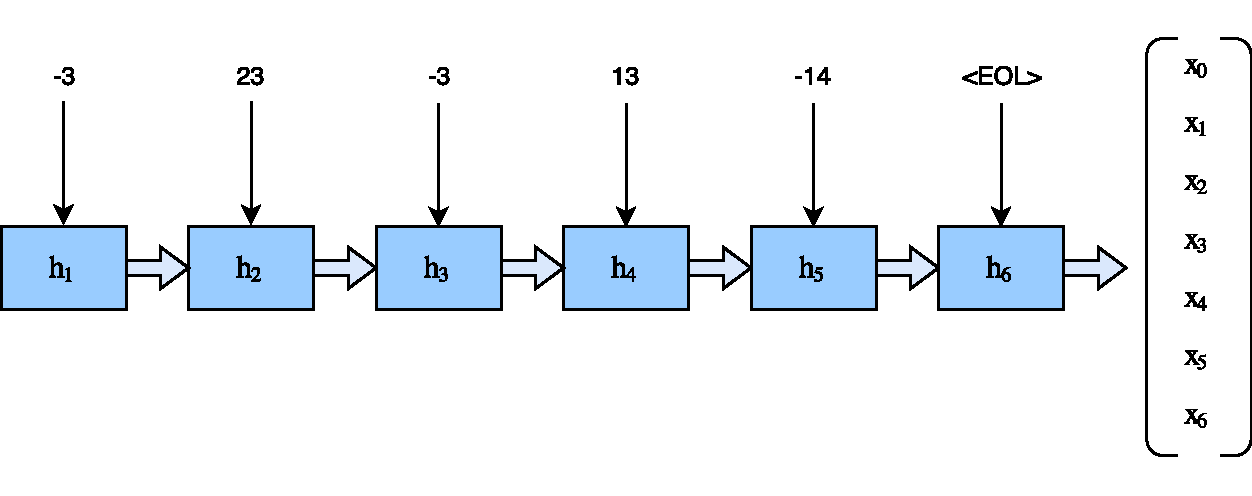
\includegraphics[width=0.7\textwidth]{fig/development_process/lstm-vector-projection-encoder.pdf}
    \caption{A LSTM outputting its final hidden state after reading a sequence}
    \label{fig:lstm-vector-projection-encoder}
\end{figure}

Figure \ref{fig:lstm-vector-projection-encoder} illustrates a regular LSTM that reads an input sequence and output its final hidden state. The output vector has a length equal to the width of the LSTM. As illustrated in Figure \ref{fig:lstm-vector-projection-decoder}, the hidden state from the LSTM is repeated \(n\) times, where \(n\) is the length of the output sequence. In this example, out output has a length of three characters, plus a special ``end of line" character. The resulting matrix of the repeated vector is then fed to another LSTM that reads each time step and output its hidden state for each iteration.

\begin{figure}[ht]
    \centering
    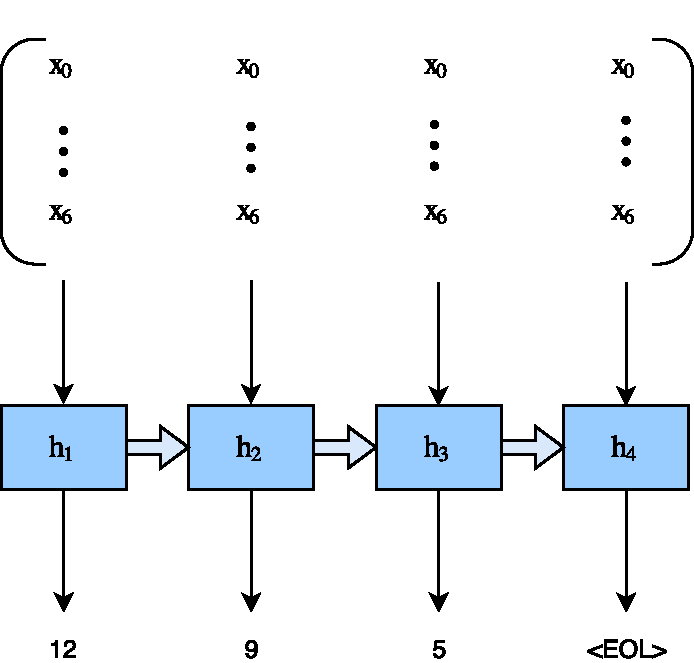
\includegraphics[width=0.5\textwidth]{fig/development_process/lstm-vector-projection-decoder.pdf}
    \caption{Repeating the output from a LSTM and feeding it to another LSTM}
    \label{fig:lstm-vector-projection-decoder}
\end{figure}

The vector approach is different from the one described in the previous iteration, and does not suffer from the same problem with alignment. Because we read the entire input sequence before anything is outputted, we no longer output anything that is dependent on data in future time steps. The vector from the first LSTM has essentially encoded the temporal dependencies in a single representation vector. This is not that different from how encoder-decoders create their fixed width context vector. The main difference between this approach and general encoder-decoders is that the output in the last LSTM is not fed back as input. This may cause problems because the output is not only dependent on the encoded input sequence, but also what it has already outputted.